% - - - - - - - - - - Appendices - - - - - - - - - - - - - -
%
%
%- - - - - - - -  Grassmann numbers  - - - - - - - - - -
%
%
%
\chapter{Grassmann Numbers}
\section{Grassmann algebra}
When we start considering a QFT including fermions, we have to conclude that our canonical quantisation rules for bosons no longer apply. Instead of a commutation relation
\begin{equation}
\left[ \phi(x),\Pi(y)\right] = i \hbar \delta(x-y)
\end{equation}
for bosonic fields, one has to introduce anticommutation relations for fermionic ones \cite{Cartier:2002zp}
\begin{equation}
\left\lbrace \psi(x),\pi(y) \right\rbrace = i \hbar \delta(x-y),
\end{equation}
which in the classical limit $\hbar \rightarrow 0$ is leading to objects that behave like anticommuting numbers
\begin{equation}
\psi\pi = -\pi\psi,
\end{equation}
which seems rather strange at first. But the concept of anticommuting numbers, so called \names{Grassmann} variables, has proved quite useful in the path integral framework to represent the algebra of fermionic position and momentum observables as operators on a space of functions. In the following we want to define these objects and study their properties.\\[1cm]
%
%
We can identify \names{Grassmann} numbers with elements of the exterior algebra $\Lambda^{1}(V)$ over a vector space $V$ over a field $K$. According to the dimension of $V$ the algebra has a finite collection of generators $\xi_{1},\ldots,\xi_{N}$ with $N=\text{dim}V \geq 1$ or infinitely many, if the vector space is infinite dimensional. With the exterior product there exists an associative connection on the algebra, which is linear in scalar multiplication and satisfies
\begin{equation}
\xi_{i}\wedge \xi_{i} =0.
\label{wedge_zero}
\end{equation}
Thereby follows the demanded anticommutativity for the fermionic \names{Grassmann} variables
\begin{equation}
\xi_{i}\wedge\xi_{j} = - \xi_{j}\wedge\xi_{i}.
\end{equation}
In general we can write the exterior algebra as a direct sum of subalgebras
\begin{equation}
\Lambda(V)=\bigoplus_{m=0}^{N} \Lambda^{m}(V),
\end{equation}
where $\Lambda^{m}(V)$ is the quotient algebra of the tensor algebra $T^{m}(V)$ and the two-sided ideal $I^{m}(V)$ and $\Lambda^{0}(V)=K$. For an $a \in \Lambda^{k}(V)$ and $b \in \Lambda^{l}(V)$ we have a graded commutative exterior product
\begin{equation}
a\wedge b = (-1)^{kl} b\wedge a.
\end{equation}
Therefore if we have an $a=\xi_{i}\wedge\xi_{j}$ and $b=\xi_{m}\wedge\xi_{n}$, then we get
\begin{equation}
a \wedge b = b \wedge a
\end{equation}
and $a$ and $b$ behave like bosonic quantities. The highest alternating tensor one can create is
\begin{equation}
\xi_{1}\wedge\xi_{2}\wedge \ldots\wedge \xi_{N} \in \Lambda^{N}(V),
\end{equation}
and with (\ref{wedge_zero}) it applies for all higher tensor spaces that $\Lambda^{k}(V)=0,\; \forall\; k>N$. From now on we want to abbreviate the wedge notation simply by
\begin{equation}
\xi_{i}\xi_{j} \equiv \xi_{i}\wedge\xi_{j}.
\end{equation}
So any analytic function of some real quantities $x_{i} \in \mathbb{R}$ and \names{Grassmannian} generators $\xi_{j} \in \Lambda(V)$ can be represented by finitely many terms
\begin{equation}
f(x_{1},\ldots,x_{n},\xi_{1},\ldots,\xi_{N}) = f_{0} + f_{1}\;\xi_{1} +\ldots+ f_{12}\;\xi_{1}\xi_{2} +\ldots+ f_{1\ldots N}\; \xi_{1}\cdots\xi_{N},
\end{equation}
where the coefficients are functions of the real quantities. In scope of this thesis we have to deal with vectors of four complex \names{Grassmann} variables and adapt our notation to the one used in \cite{Giombi:2009gd}
\begin{equation}
\eta_{i} =\frac{1}{\sqrt{2}} \left(\xi\R_{i} +i\,\xi\I_{i}\right),\qquad \text{with} \quad \xi\R_{i},\xi\I_{i} \in \Lambda^{1}(V), \quad i=(1,\ldots,4).
\end{equation}
We now define the \names{Grassmann} variables with an upper index as the complex conjugate of the ones with lower index $\eta^{i}\equiv \left(\eta_{i}\right)^{\dagger} = \left(\eta_{i}\right)^{\ast}$. Complex conjugation of two real \names{Grassmann} numbers is defined to include a change of position
\begin{equation}
\left(\xi_{1}\xi_{2}\right)^{\ast}\equiv \xi_{2}^{\ast}\xi_{1}^{\ast} = -\xi_{1}\xi_{2}.
\end{equation}
They therefore behave like a formally purely imaginary quantity, whereas
\begin{equation}
\left(i\xi_{1}\xi_{2}\right)^{\ast} = i\xi_{1}\xi_{2}
\end{equation}
behaves like a formally real quantity.
%
%
%
%
%
%    GRASSMANN ANALYSIS
%
%
%
%
\section{Grassmann analysis} \label{sec: grassmann_analysis}
Now we want to see how we can differentiate and integrate \names{Grassmann} variables. We define the derivative to be
\begin{equation}
\dfrac{\del \xi_{m}}{\del\xi_{n}}\equiv\delta_{m n} .
\end{equation}
Following \cite{Cartier:2002zp} and \cite{Berezin} we define the product rule to satisfy
\begin{align}
\dfrac{\del }{\del\xi_{n}} \left(\xi_{m_{1}}\xi_{m_{2}}\cdots \xi_{m_{r}}\right) &\equiv \delta_{m_{1} n}\,\xi_{m_{2}}\cdots\xi_{m_{r}}-\delta_{m_{2} n}\,\xi_{m_{1}} \xi_{m_{3}}\cdots \xi_{m_{r}} +\cdots  \notag \\
&\quad + (-1)^{r-1} \delta_{m_{r} n}\,\xi_{m_{1}}\cdots \xi_{m_{r}}.
\end{align}
The tangent vectors are also elements of the exterior algebra and satisfy the same anticommutation rules
\begin{equation}
\frac{\del }{\del \xi_{i}} \frac{\del }{\del\xi_{j}} = - \frac{\del }{\del \xi_{j}} \frac{\del }{\del\xi_{i}}.
\end{equation}
%
%
So if we perform a coordinate transformation $\xi_{i}=M_{ij}\,\theta_{j}$, an $n$-form is transforming according to the alternating properties of forms like
\begin{equation}
\frac{\del }{\del \xi_{1}}\cdots\frac{\del }{\del \xi_{n}} = \mathrm{det}\left(M^{-1}\right) \frac{\del }{\del \theta_{1}}\cdots \frac{\del }{\del \theta_{n}},
\label{coord_trafo}
\end{equation}
where the matrix $M$ is associated with the \names{Jacobian}
\begin{equation}
M_{ij}=\frac{\del \xi_{i}}{\del\theta_{j}}.
\end{equation}
For an integral $\mathcal{I}[f]$ of a function $f(\xi)$ it holds true that
\begin{equation}
\dfrac{\del}{\del \xi}\mathcal{I}[f] =0,
\end{equation}
since the integral is independent of the integration variable. With (\ref{wedge_zero}) it is also true that
\begin{equation}
\dfrac{\del}{\del \xi}\dfrac{\del}{\del \xi}=0
\end{equation}
and therefore one can identify the integration on \names{Grassmann} numbers with the differentiation up to some normalization constant $C$
\begin{equation}
\mathcal{I}[f]=\int \dd\xi\; f(\xi) = C\frac{\del }{\del\xi}f(\xi).
\end{equation}
So we end up with the following integration rules, if we define $C\equiv 1$:
\begin{equation}
\int \dd\xi\; \xi = \frac{\del }{\del\xi}\xi =1,\qquad \int \dd\xi\; 1 = \frac{\del }{\del\xi}1 =0.
\end{equation}
We now want to perform an integration over the complex \names{Grassmann} variables $\eta$ and $\eta^{\dagger}$. Therefore we want to investigate an integration over the function
\begin{equation}
e ^{-a\eta\eta^{\dagger}}.
\end{equation}
With
\begin{equation}
\eta\eta^{\dagger} = \frac{1}{2}\left(\xi\dR+i\,\xi\dI\right)\left(\xi\dR-i\, \xi\dI\right) = -i\,\xi\dR\xi\dI
\end{equation}
and (\ref{coord_trafo}) we can transform the integral using that the determinant of the \names{Jacobian} is $\mathrm{det}\,J=i$ and find
\begin{align}
\int \dd\eta\dd\eta^{\dagger}\;e ^{-a\eta\eta^{\dagger}} &= i\int \dd\xi\dR \dd\xi\dI\; e ^{ia\xi\dR\xi\dI}\notag \\
%
%
&=i\int\dd\xi\dR\dd\xi\dI\, \left( 1+ i\,a\xi\dR\xi\dI \right) \\
%
%
&=a \int\dd\xi\dR\dd\xi\dI \;\xi\dI\xi\dR = a \notag
\end{align}
We get the same result by integrating over two real \names{Grassmann} variables $\xi_{1}$ and $\xi_{2}$
\begin{equation}
\int \dd\xi_{1}\dd\xi_{2}\; e ^{-a\xi_{1}\xi_{2}}=a.
\end{equation}
By rewriting it with help of the antisymmetric matrix
\begin{equation}
A=\left(\begin{array}{cc}
0 & a \\
-a & 0
\end{array} \right)
\end{equation}
we get
\begin{equation}
\int \dd\xi_{1}\dd\xi_{2}\; e ^{-\frac{1}{2}\xi_{i}A_{ij}\xi_{j}} = \mathrm{Pf}\left(A\right),
\end{equation}
where $\mathrm{Pf}\left(A\right)$ is the \names{Pfaffian} of $A$, which is defined by the factorisation of the determinant in the following way
%
%
\begin{equation}
\mathrm{Pf}\left(A\right)^{2} = \det(A)
\end{equation}
This relation holds true for an even number of arbitrary many \names{Grassmann} generators. Its is therefore possible to integrate out \names{Grassmann} variables and be left with calculating a determinant or \names{Pfaffian}, which comes in quite essential when dealing with \names{Grassmann} integrals numerically.
%
%
%
%
% HUBBARD-STRATONOVICH TRAFO
%
%
%
%
\section{Hubbard-Stratonovich transformation} \label{sec: HS_trafo}
We have now seen how to deal with bilinear exponentials. But in many cases one also has to deal with higher forms than bilinears. In principle one can expand any function into finitely many terms, like we have seen earlier, and then perform the integration rules, which is but rather ugly and proved not very efficient in numerical simulations. But there is a method to transform an exponential with 4-forms into one with bilinears, by performing an integration over additional bosonic auxiliary fields. This is called a \names{Hubbard-Stratonovich} transformation. Assuming that we have a finite number of complex \names{Grassmann} variables $\eta_{i}$, we can see that the object $\eta^{2}\equiv \eta^{i}\eta_{i}$ transforms like a formally real quantity
\begin{equation}
\left(\eta^{i}\eta_{i}\right)^{\ast}=\left(\eta_{i}\right)^{\ast}\left(\eta^{i}\right)^{\ast} =\eta^{i}\eta_{i}.
\end{equation}
Therefore $\left(\eta^{2}\right)^{2}$ is a formally positive real value and we can apply the identity
\begin{equation}
e ^{\frac{(\eta^{2})^{2}}{4a}}=\sqrt{\frac{a}{\pi}} \int\dd\phi\;e ^{-a\phi^{2}+\eta^{2}\phi},
\label{HST_pos}
\end{equation}
which one can proof simply by square addition and performing a \names{Gaussian} integral. If we see this identity in the context of the path integral  framework, we can say, that a new bosonic auxiliary field $\phi$ is introduced for the specific space time point, where the integration took place. Since we can do this transformation at every space time point, this leads to a whole path integral  over $\phi$. Now we also have to be aware of what happens if the exponent on the left side of (\ref{HST_pos}) is negative
\begin{equation}
e ^{-\frac{(\eta^{2})^{2}}{4a}}=e ^{\frac{(i\eta^{2})^{2}}{4a}}=\sqrt{\frac{a}{\pi}} \int\dd\phi\; e ^{-a\phi^{2}+i\eta^{2}\phi}.
\end{equation}
We can see that this introduces an imaginary term in the exponent and therefore a high oscillatory function in the integral. Analytically this term would not bother us, but since we want to perform a numerical calculation something like this often results into a numerical sign problem, discussed in section \ref{sec: sign_prob}.

%
%
% - - - - - - -  AdS spacetime - - - - - - - - - - - - -
%
%
%
\chapter[$\mathbf{AdS_{5}\times S^{5}}$ spacetime]{$\mathitbf{AdS_{5}\times S^{5}}$ spacetime}%[$AdS_{5}\times S^{5}$ spacetime]
The $AdS_{5}\times S^{5}$ space is in the central focus of the gauge/gravity duality and should be concerned more deeply. It is a direct product of five dimensional Anti-de Sitter ($AdS$) space and a five dimensional compact sphere. Both are maximally symmetric spaces and therefore inherit the isometry groups $SO(2,4)$ in case of $AdS_{5}$ and respectively $SO(6)$ for $S^{5}$ \cite{Ammon:2015wua}. This is an important fact for the $AdS/CFT$ correspondence since the direct product of these groups has the same amount of degrees of freedom as the superconformal group $SO(2,4)\times SO(6) = SU(2,2\vert 4)$ as the undelying symmetry group of $\mathcal{N}=4$ super \names{Yang-Mills} theory in four dimensional \names{Minkowski} space.
%
%
\section[$\mathrm{AdS_{5}}$ space]{$\mathitbf{AdS_{5}}$ space}\label{AdS5}
Since the construction of a sphere is rather simple, we focus on the Anti-de Sitter space. $AdS_{5}$ is a hyperboloid with constant negative curvature, that can be embedded in six dimensional \names{Minkowski} spacetime $X = (X^{0},X^{1},\ldots,X^{5}) \in \mathbb{R}^{4,2}$, with metric ${\tilde{\eta} = {\rm diag}(-,+,+,+,+,-)}$, so that
\begin{equation}
\dd s^{2} = -\left(\dd X^{0}\right)^{2} + \left(\dd X^{1}\right)^{2} + \cdots + \left(\dd X^{4}\right)^{2} - \left(\dd X^{5}\right)^{2} = \tilde{\eta}_{MN} \dd X^{M}\dd X^{N},
\end{equation}
where $M,N \in {0,\ldots,5}$. $AdS_{5}$ is then given by the hypersurface
\begin{equation}
\tilde{\eta}_{MN}X^{M}X^{N} = -\left(X^{0}\right)^{2} + \left(X^{1}\right)^{2} + \cdots + \left(X^{4}\right)^{2} - \left(X^{5}\right)^{2} = -R^{2},
\label{hyperbol}
\end{equation}
%
%
\begin{figure}[ht!]
\begin{center}
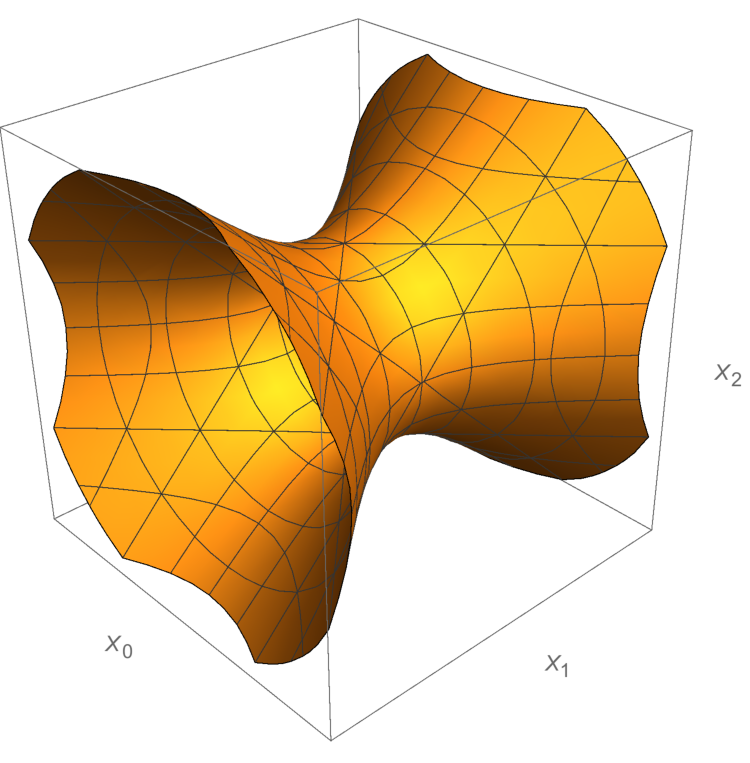
\includegraphics[width=0.6\textwidth]{AdS2.pdf}
\caption{Embedding of $AdS_{2}$ in $\mathbb{R}^{3}$ as a hypersurface given by the equation $-(X_{0})^{2}+(X_{1})^{2}-(X_{3})^{2}=-1$. \label{fig: AdS2}}
\end{center}
\end{figure}
%
%
where $R$ is the radius of curvature of the $AdS_{5}$ space, see also \autoref{fig: AdS2}  for an embedding of $AdS_{2}$ in $\mathbb{R}^{3}$. For large $X^{M}$ the hyperboloid approaches the light-cone of the \names{Minkowski} space $\mathbb{R}^{4,2}$, given by
\begin{equation}
\tilde{\eta}_{MN}X^{M}X^{N} = 0.
\label{M_l_c}
\end{equation}
We therefore can define the `boundary' $\del AdS_{5}$ of Anti-de Sitter space by the set of all lines on the light-cone (\ref{M_l_c}) originating from $0 \in \mathbb{R}^{4,2}$. For a point $X \neq 0$ in $AdS_{5}$ close to the boundary and therefore satisfying (\ref{M_l_c}) we can define $(u,v)$ by
\begin{equation}
u = X^{5}+X^{4}, \qquad v = X^{5}-X^{4},
\end{equation}
so we can rewrite (\ref{M_l_c}) as
\begin{equation}
uv = \eta_{\mu \nu} X^{\mu}X^{\nu},
\end{equation}
with $\mu,\nu \in {0,1,2,3}$ and $\left(\eta_{\mu \nu}\right) = {\rm diag}(-,+,+,+).$ Whenever $v \neq 0$ we can rescale the coordinates to set $v = 1$ and solve for $u$. Therefore one is left with a four dimensional \names{Minkowski} space $\mathbb{R}^{3,1}$. Points with $v=0$ are ``points at infinity'' added to four dimensional \names{Minkowski} space. This makes $\del AdS_{5}$ a conformal compactification of four dimensional \names{Minkowski} space. According to Maldacena \cite{maldacena1} the correspondence between a $\mathcal{N}=4$ theory on $\mathbb{R}^{3,1}$ and Type IIB on $AdS_{5}\times S^{5}$ therefore expresses a string theory on $AdS_{5}\times S^{5}$ in terms of a theory on the boundary and thus is referred to as ``holographic'' \cite{Witten:1998qj}.
%
%
\section{Poincaré patch}\label{p_patch}
Let us now introduce a parametrisation of the hyperboloid (\ref{hyperbol}) by the following coordinates $x^{\mu} \in \mathbb{R}$, for $\mu \in {0,1,2,3}$ and $z \in \mathbb{R}_{+}$. The parametrisation in these coordinates is given by (see e.g. \cite{Ammon:2015wua,Bayona:2005nq})
\begin{align}
X^{0} &= \frac{z}{2} \left( 1+ \frac{1}{z^{2}}\left( x_{\mu}x^{\mu} + R^{2}\right) \right), \notag \\
X^{i} &= \frac{R}{z}x^{i},\quad i\in {1,2,3}, \\
X^{4} &= \frac{z}{2} \left( 1 + \frac{1}{z^{2}} \left(x_{\mu}x^{\mu} -R^{2} \right) \right), \notag \\
X^{5} &= \frac{R}{z}x^{0}, \notag
\end{align}
with $x_{\mu}x^{\mu}=\eta_{\mu\nu}x^{\mu}x^{\nu}$ and $\left(\eta_{\mu \nu}\right) = {\rm diag}(-,+,+,+)$. These local coordinates are called \names{Poincaré} patch. The metric of $AdS_{5}$ in the \names{Poincaré} patch reads
\begin{equation}
\dd s^{2} = \frac{R^{2}}{z^{2}}\left(\dd z^{2} + \eta_{\mu \nu} \dd x^{\mu} \dd x^{\nu} \right).
\end{equation}
%
%
For the whole $\AdSS$ space in \names{Poincaré} patch we find
%
%
\begin{equation}
\dd s^{2} = \frac{R^{2}}{z^{2}}\left(\dd z^{2} + \eta_{\mu \nu} \dd x^{\mu} \dd x^{\nu} \right) + \dd u^{I}\dd u^{I},
\end{equation}
%
%
where $u^{I}$ $(I=1,\ldots,6)$ are coordinates on $S^{5}$ that satisfy $u^{I}u^{I}=R^{2}$. For $z\to 0$ we approach the boundary of $\AdSS$ and we can see from the metric that the contribution of the sphere becomes neglectable close to the boundary. If we include the infinite regime as $\del (\AdSS)$ where $z=0$ we can convince ourselves that the metric is conformally equivalent to 4d \names{Minkowski} space.
%
%
%
%- - - - - - - - - rho matrix conventions - - - - - - - - - - - - -
%
%
%
\chapter{SO(6) matrices} \label{sec: SO6}
The matrices $\rho^{M}_{ij}$ appearing in the action (\ref{eq: cusp_action}) are the off-diagonal blocks of $SO(6)$ \names{Dirac} matrices $\gamma^{M}$ in chiral representation\footnote{The upper or lower placement of the index $M$ on the block matrices has no meaning and is only changed for the purpose of readability.}
%
%
\begin{equation}
\gamma^{M} \equiv \begin{pmatrix}
0 & \rho_{M}^{\dagger} \\
\rho^{M} & 0
\end{pmatrix}
= \begin{pmatrix}
0 & (\rho^{M})^{ij} \\
(\rho^{M})_{ij} & 0
\end{pmatrix} .
\end{equation}
%
%
The $\rho^{M}_{ij}$ shall all skew symmetric and we define the ones with the upper indices to satisfy $(\rho^{M})^{ij}\equiv (\rho^{M}_{ij})^{\dagger}$. We can therefore state the following properties
%
%
\begin{equation}
\rho^{M}_{ij}= - \rho^{M}_{ji}, \qquad  (\rho^{M})^{ij} = - (\rho ^{M}_{ij})^{*},
\end{equation}
%
%
and we chose to use the following representation
%
%
\begin{align}
\rho^{1}_{ij} &= \begin{pmatrix}
0 & 1 & 0 & 0 \\
-1 & 0 & 0 & 0 \\
0 & 0 & 0 & 1 \\
0 & 0 & -1 & 0
\end{pmatrix} , &
%
\rho^{2}_{ij} &= \begin{pmatrix}
0 & i & 0 & 0 \\
-i & 0 & 0 & 0 \\
0 & 0 & 0 & -i \\
0 & 0 & i & 0
\end{pmatrix} , &
%
\rho^{3}_{ij} &= \begin{pmatrix}
0 & 0 & 0 & 1 \\
0 & 0 & 1 & 0 \\
0 & -1 & 0 & 0 \\
-1 & 0 & 0 & 0
\end{pmatrix} , \notag\\[0.6cm]
%
%
%
\rho^{4}_{ij} &= \begin{pmatrix}
0 & 0 & 0 & -i \\
0 & 0 & i & 0 \\
0 & -i & 0 & 0 \\
i & 0 & 0 & 0
\end{pmatrix} , &
%
\rho^{5}_{ij} &= \begin{pmatrix}
0 & 0 & i & 0 \\
0 & 0 & 0 & i \\
-i & 0 & 0 & 0 \\
0 & -i & 0 & 0
\end{pmatrix} , &
%
\rho^{6}_{ij} &= \begin{pmatrix}
0 & 0 & 1 & 0 \\
0 & 0 & 0 & -1 \\
-1 & 0 & 0 & 0 \\
0 & 1 & 0 & 0
\end{pmatrix} . \raisetag{-6pt}
\end{align}
%
%
From the \names{Clifford} algebra of the \names{Dirac} matrices $\lbrace \gamma^{M}, \gamma^{N}\rbrace = 2\delta^{MN}\mathds{1}_{8}$ we can derive the relation
%
%
\begin{equation}
(\rho^{M})^{il} (\rho^{N})_{lj} + (\rho^{N})^{il}(\rho^{M})_{lj} = 2\delta^{MN}\delta^{i}_{j}.
\end{equation}
%
%
The generators of the $SO(6)$ can be built by
%
%
\begin{equation}
{\left(\rho^{MN}\right)^{i}}_{j} = \frac{1}{2} \left[ \left(\rho^{M}\right)^{il} \left(\rho^{N}\right)_{lj} - \left(\rho^{N}\right)^{il} \left(\rho^{M}\right)_{lj} \right].
\end{equation}
%
%
Further relations and identities are
%
%
\begin{align}
{\left(\rho^{MN}\right)^{i}}_{j} &= {\left(\rho^{MN}\right)^{*}_{i}}^{j}\;, & {\left(\rho^{MN}\right)^{i}}_{j} &= {\left(\rho^{NM}\right)_{j}}^{i}\;,
\label{eq: SO6_id} \\
 (\rho^M)^{im} (\rho^M)^{kn}&=2\epsilon^{imkn}\;, &  (\rho^M)^{im} (\rho^M)_{nj}&=2\left(\delta^i_j \delta^m_n -\delta^i_n \delta^m_j\right)\;,
\end{align}
%
%
\begin{align}
 &\quad \epsilon^{imkn} (\rho^M)_{mj}(\rho^L)_{nl}+\epsilon_{mjnl}(\rho^M)^{im}(\rho^L)^{kn}\\
 &=(\rho^{\{M})^{ik}(\rho^{L\}})^{jl}+\delta^k_j(\rho^L)^{im}(\rho^M)_{ml}+\delta^i_l(\rho^M)^{km}(\rho^L)_{mj}\nonumber \\
 &\quad+\delta^{ML}\left(-4\delta^i_l \delta^k_j +2\delta^i_j\delta^k_l\right)\;,\nonumber\\[0.4cm]
& -{(\rho^{MN})^i}_j {(\rho^{ML})^k}_l n_N n_L=-2(\rho^{N})^{ik} (\rho^{L})_{jl} n_N n_L-\delta^i_j \delta^k_l+2\delta^i_l \delta^k_j \;.
\end{align}
%
%
%
%
%- - - - - - - - - Discrete Fourier Transform - - - - - - - - - -
%
%
%
\chapter{Discrete Fourier Transform}
\label{app: disc_ft}
To perform a Fourier transform on the lattice one needs to discretize it to deal with a finite sequence of $N$ complex numbers $x_{0},x_{1},\ldots,x_{N-1}$. We define the discrete Fourier transform $X_{k}$ to be a vector in the base of roots of unit with components $x_{n}$ as follows:
\begin{equation}
X_{k}=\dfrac{1}{\sqrt{N}} \sum\limits_{n=0}^{N-1} x_{n} \, e ^{-2\pi  i kn /N} \qquad  k \in \mathbb{Z}.
\label{FT}
\end{equation}
We can limit the domain of $k$ to a finite set, because the exponential is periodic in $k$. In the following we want to stick to the domain $k \in \left[ -\tfrac{N}{2}+1,\ldots,\tfrac{N}{2} \right]$ and restrict us to even $N$. The inverse transform can be defined to be
%
\begin{equation}
 x_{n}= \dfrac{1}{\sqrt{N}} \sum\limits_{k=-N/2+1}^{N/2} X_{k} \, e ^{2 \pi  i nk /N},
 \label{invFT}
 \end{equation}
 where due to periodicy $n$ is in the domain $\left[0,\ldots,N-1\right]$ like defined in the beginning. If we now insert (\ref{FT}) into (\ref{invFT}) we end up with
\begin{align}
x_{n} &=\dfrac{1}{N}\sum\limits_{k=-N/2+1}^{N/2} \left( \sum\limits_{m=0}^{N-1} x_{m}  e ^{-2\pi  i km /N} \right)  e ^{2\pi  i kn /N} \\
%
%
&= \dfrac{1}{N} \sum\limits_{k',m=0}^{N-1} x_{m}  e ^{2\pi  i k'(n-m) /N},
\end{align}
where we shifted the summation for $k'$ to be in the same domain as $m$. This is now only equal to $x_{n}$ if the following important relation holds true
%
%
\begin{equation}
\dfrac{1}{N} \sum\limits_{k'=0}^{N-1}  e ^{2\pi  i k'(n-m) /N} = \delta_{m,n}.
\end{equation}
We can prove this easily. For $n=m$ this is trivial and for $n\neq m$ we make use of the geometric series
\begin{equation}
\sum\limits_{k'=0}^{N-1} \left( e ^{2\pi i  c/N }\right)^{k'} = \dfrac{1- e ^{2\pi i  c}}{1- e ^{2\pi i  c/N }} = 0, \qquad  \vert c\vert = \vert n-m \vert \in [1,\ldots,N-1].
\end{equation}
%
%
Now we want to apply the Fourier transform on the two dimensional lattice used throughout this thesis. We defined the lattice to be
\begin{equation}
\mathit{\Lambda}=\left\lbrace  n=\left(n_{0},n_{1}\right) \vert n_{0}=1,\ldots,N_{0}\,; \; n_{1}=1,\ldots,N_{1} \right\rbrace,
\end{equation}
with $N_{0}=T$ and $N_{1}=L$. Therefore the total number of lattice points is given by
\begin{equation}
\vert \mathit{\Lambda}\vert \equiv TL.
\end{equation}
Following \cite{gattringer2009quantum} we now want to calculate the discrete Fourier transform $\tilde{f}(p)$ of a function $f(n)$. Here for $f(n)$ we impose toroidal boundary conditions
\begin{equation}
f(n+\hat{\imath}N_{i})= e ^{2\pi i \theta_{i}}f(n),
\label{eq: boundary_cond}
\end{equation}
where $\hat{\imath}$ is a unit vector in the $i$-direction and $\theta_{i}=0$ corresponds to periodic and $\theta_{i}=1/2$ to anti-periodic boundary conditions. The discrete momentum space corresponding to these boundary conditions is given by
\begin{equation}
\mathit{\widetilde{\Lambda\,}}= \left\lbrace p=(p_{0},p_{1}) \vert\, p_{i}=\dfrac{2\pi}{aN_{i}}(k_{i}+\theta_{i}) ,\, k_{i}=-\dfrac{N_{i}}{2}+1,\ldots,\dfrac{N_{i}}{2} \right\rbrace.
\end{equation}
With (\ref{FT}) and (\ref{invFT}) we can express the the Fourier transform as
\begin{equation}
\tilde{f}(p)=\dfrac{1}{\sqrt{\vert\mathit{\Lambda}\vert}} \sum\limits_{n\in \mathit{\Lambda}} f(n)\,  e ^{- i  p\cdot na}
\end{equation}
and for the inverse transform we find
\begin{equation}
f(n) = \dfrac{1}{\sqrt{\vert\mathit{\Lambda}\vert}} \sum\limits_{p\in \widetilde{\mathit{\Lambda}\,}} \tilde{f}(p)\,  e ^{ i p\cdot na}.
\end{equation}
Here again the important relations hold
\begin{align}
\dfrac{1}{\vert\mathit{\Lambda}\vert} \sum\limits_{n\in \mathit{\Lambda}} \text{exp}( i (p-p')\cdot na) &=\delta(p-p') \equiv \delta_{k_{0},k'_{0}}\delta_{k_{1},k'_{1}} \\
\dfrac{1}{\vert\mathit{\Lambda}\vert} \sum\limits_{p\in  \widetilde{\mathit{\Lambda}\,}} \text{exp}( i p\cdot (n-n')a) &=\delta(n-n') \equiv \delta_{n_{0},n'_{0}}\delta_{n_{1},n'_{1}}.
\end{align}
%
%
%
%
%
%
% - - - -  -- - - - - - - - -   discretized fermion matrix  - - - - - - - - - - - - - - - -
%
%
%
%
%
\chapter{Discretized fermion matrix}
\label{app: disc_ferm}
Here we want to present the details leading to the discretized version (\ref{eq: disc_OF}) of the operator $\mathcal{O}_{\rm F}$. As emphasized in section \ref{sec: ferm_op} $\hat{\mathcal{O}}_{\rm F}$ is a $16V\times 16V$ matrix and we will continue to use the notation introduced there to write subdivided blocks of size $4V\times 4V$ to result in
%
%
\begingroup
\everymath{\footnotesize}
\begin{flalign}
\!
\hat{\mathcal{O}}_{\rm F} =
\begin{pmatrix}
\hat{W}_{+} & i\bar{\Delta}^{\rm A}_{0} & -i\left(\vec{\Delta}^{Z}_{1} + \tfrac{M}{2}\bar{Z}\right) & 0 \\
i\bar{\Delta}^{\rm A}_{0} & -\hat{W}_{+}^{\dagger} & 0 & -i\left(\vec{\Delta}^{Z^{\dagger}}_{1} + \tfrac{M}{2}\bar{Z}^{\dagger}\right)  \\
i\left(\cev{\Delta}^{Z}_{1} - \tfrac{M}{2}\bar{Z}\right)  & 0 & \!\!\!\!\!\!\!\!\! 2\left(\bar{\Delta}^{x}_{1}-\tfrac{M}{2}\bar{Z}^{x}\right)+\hat{W}_{-} & i\bar{\Delta}^{\rm A}_{0} -\hat{A}^{\rm T} \\
0 & i\left(\cev{\Delta}^{Z^{\dagger}}_{1} - \tfrac{M}{2}\bar{Z}^{\dagger}\right) & i\bar{\Delta}^{\rm A}_{0} +\hat{A} & \!\!\!\!\! 2\left(\bar{\Delta}^{x^{*}}_{1}-\tfrac{M}{2}\bar{Z}^{x^{*}}\right)-\hat{W}_{-}^{\dagger}
\end{pmatrix} .
\raisetag{-8pt}
\end{flalign}
\endgroup
%
%
First of all we should mention that the operator $\mathcal{O}_{\rm F}$ was of dimension $[a]^{-1}$ which has been absorbed into the fermionic fields to make them dimensionless. Therefore $\hat{\mathcal{O}}_{\rm F}$ is dimensionless as well, as are now all the bosonic and fermionic fields. Further $\hat{\mathcal{O}}_{\rm F}$ needs to be anti-symmetric which is why all the discretized derivatives need to be symmetric finite differences. As it is standard in lattice QCD to use anti-periodic boundary conditions in the temporal direction for the fermions \cite{montvay_lattice}, we will apply those here as well. For the spacial direction periodic boundary conditions shall be used. So starting from block $(1,2)$ we make the transition
%
%
\begin{equation}
i \del_{t}\mathds{1}_{4} \longrightarrow i \bar{\Delta}^{\rm A}_{0},
\end{equation}
%
%
where we defined
%
%
\begin{align}
\bar{\Delta}^{\rm A}_{0} &\equiv \bar{\Delta}^{\rm a}_{0} \otimes \mathds{1}_{4}, &
\bar{\Delta}^{\rm a}_{0} &\equiv \left(\bar{\Delta}^{\rm a}_{0}\right)(l,p) = \frac{1}{2}\left( \delta_{l_{+\hat{1}},p}^{\rm a}-\delta_{l_{-\hat{1}},p}^{\rm a}\right).
\end{align}
%
%
Thereby the superscripts \textit{A, a} refer to the property of the finite differences to respect anti-periodic boundary conditions, whereas \textit{p} will refer to periodic ones. In the next block $(1,3)$ we have
%
%
\begin{equation}
-i \rho^{M}\left(\del_{s} +\tfrac{m}{2}\right) \frac{z^{M}}{z^{3}} \longrightarrow -i \left( \vec{\Delta}_{1}^{Z} +\tfrac{M}{2} \bar{Z}\right).
\end{equation}
%
%
Since $z^{M}/z^{3}$ is on the right, the derivative will also act on this term which we will have to consider in the discretization. Thus we introduce the definitions
%
%
\begin{gather}
Z \equiv Z_{ij}(l) = \rho_{ij}^{M} \frac{z^{M}(l)}{z^{3}(l)}, \qquad \bar{Z} \equiv \bar{Z}_{ij}(l,p) = \delta_{l,p} Z_{ij}(l), \\
\vec{\Delta}_{1}^{Z} \equiv \left(\vec{\Delta}_{1}^{Z}\right)_{ij}(l,p) = \frac{1}{2} \left[ \delta_{l_{+\hat{1}},p}^{\rm p}Z_{ij}(l_{+\hat{1}})-\delta_{l_{-\hat{1}},p}^{\rm p} Z_{ij}(l_{-\hat{1}})\right].
\end{gather}
%
%
The right arrow shall indicate that $Z$ is on the right and respected by the derivative. In block $(3,1)$ we also have the same operator with arrow to the left which indicates that the derivative will not act on $Z$
%
%
\begin{equation}
\cev{\Delta}_{1}^{Z} \equiv \left(\cev{\Delta}_{1}^{Z}\right)_{ij}(l,p) = \frac{1}{2} \left[ \delta_{l_{+\hat{1}},p}^{\rm p}-\delta_{l_{-\hat{1}},p}^{\rm p}\right] Z_{ij}(l) .
\end{equation}
%
%
In block $(3,3)$ we observe
%
%
\begin{equation}
2\frac{z^{M}}{z^{4}}\rho^{M}\left(\del_{s}x-\tfrac{m}{2}x\right) \longrightarrow  2\left( \bar{\Delta}_{1}^{x}-\tfrac{M}{2}\bar{Z}^{x} \right),
\end{equation}
%
%
where
%
%
\begin{gather}
\bar{Z}^{x} \equiv \bar{Z}^{x}_{ij}(l,p) = \delta_{l,p}\frac{Z_{ij}(l)}{z(l)}x(l), \\
\bar{\Delta}_{1}^{x} \equiv \left(\bar{\Delta}_{1}^{x}\right)_{ij}(l,p) = \frac{1}{2} \frac{Z_{ij}(l)}{z(l)} \left[ \delta_{l_{+\hat{1}},p}^{\rm p}x(l_{+\hat{1}})-\delta_{l_{-\hat{1}},p}^{\rm p} x(l_{-\hat{1}})\right].
\end{gather}
%
%
The discretized version of $A$ is given by
%
%
\begin{align}
\hat{A}_{ij}(l,p) = &-\delta_{ij}\delta_{lp}\frac{\sqrt{6}}{z(l)}\phi(l) + \delta_{lp}\frac{\widetilde{\phi}_{ij}(l)}{z(l)} \notag \\
%
&+i \frac{z^{N}(l)}{z(l)} \big(\rho^{MN}\big)_{ij} \left( \delta^{\rm p}_{l_{+\hat{1}},p} z^{M}(l_{+\hat{1}}) - \delta^{\rm p}_{l_{-\hat{1}},p} Z^{M}(l_{-\hat{1}})\right) \\
%
&+ \frac{1}{z^{3}(l)} \big(\rho^{*}_{N}\big)_{ik} \widetilde{\phi}_{sk}(l) \big(\rho^{L}\big)_{sj} z^{N}(l)z^{L}(l) \delta_{lp}. \notag
\end{align}
%
%
For the other variations of the finite differences one simply substitutes $Z^{\dagger}$ or $x^{*}$ in the associated expressions to derive $\vec{\Delta}^{Z^{\dagger}}_{1}$ and $\bar{\Delta}^{x^{*}}_{1}$. Since $\hat{\mathcal{O}}_{\rm F}$ is anti-symmetric we need to meet the condition that $\vec{\Delta}^{Z}_{1}=-\big( \cev{\Delta}^{Z}_{1} \big)^{\rm T}$ which is easy to check. The same property is needed for corresponding \names{Wilson} term. One can define it to consist of two parts $\hat{W}^{(1)}_{\pm}$ and $\hat{W}^{(2)}_{\pm}$ which obey $\hat{W}^{(1)}_{\pm} = -\left( \hat{W}^{(2)}_{\pm} \right)^{\rm T}$ and vice versa. The resulting \names{Wilson} term
%
%
\begin{equation}
\hat{W}_{\pm} = \frac{1}{2}\left( \hat{W}^{(1)}_{\pm} + \hat{W}^{(2)}_{\pm} \right)
\end{equation}
%
%
is therefore skew-symmetric $\big(\hat{W}_{\pm}\big)^{\rm T} = -\hat{W}_{\pm}$ which is necessary since it is sitting on the diagonal blocks of $\hat{\mathcal{O}}_{\rm F}$. The single terms are constructed in the following way
%
%
\begin{align}
\hat{W}^{(1)}_{\pm} &= \frac{r}{2} \left[ \vec{\Lambda}^{Z}_{0} \pm i \vec{\Lambda}^{Z}_{1}\right] , &
\hat{W}^{(2)}_{\pm} &= \frac{r}{2} \left[ \cev{\Lambda}^{Z}_{0} \pm i \cev{\Lambda}^{Z}_{1}\right]
\end{align}
%
%
with
%
%
\begin{align}
Z^{z} &\equiv Z^{z}_{ij}(l) = Z_{ij}(l)z(l) \notag \\
\vec{\Lambda}^{Z}_{\alpha} &\equiv \big(\vec{\Lambda}^{Z}_{\alpha}\big)_{ij}(l,p) = 2\delta_{l,p}Z^{z}(l) - \delta_{l_{+\hat{\alpha}},p}Z^{z}(l_{+\hat{\alpha}}) - \delta_{l_{-\hat{\alpha}},p}Z^{z}(l_{-\hat{\alpha}}) \\
%
%
\cev{\Lambda}^{Z}_{\alpha} &\equiv \big(\cev{\Lambda}^{Z}_{\alpha}\big)_{ij}(l,p) = \left( 2 \delta_{l,p} -\delta_{l_{+\hat{\alpha}},p} - \delta_{l_{-\hat{\alpha}},p} \right) Z^{z}(l), \notag
\end{align}
%
%
where again the temporal finite differences need to respect anti-periodic and the spacial ones periodic boundary conditions. The actual implementation nonetheless is slightly different. There we constructed $\hat{W}_{\pm}$ to have its upper triangular matrix equal to $\hat{W}_{\pm}^{(1)}$ and the lower triangular matrix equal to $\hat{W}_{\pm}^{(2)}$ which in the end is leading to the same result.
